\section{Teknik Preprocessing}
    \subsection{Porter Algoritma}
        Stemmer yang paling sering digunakan adalah Algoritma Porter. 
        Porter Stemmer akan menghilangkan afiks dari suatu kata dengan ingkat berdasarkan semua aturan dan kondisi dari kata tersebut. 
        Karena tidak mempertimbangkan kosa kata dan arti dari kata itu sendiri maka algoritma porter sering dikira \textit{error}. 
        Kata-kata yang memiliki arti yang berbeda direduksi menjadi stem yang sama, misalnya ``\textit{generic}`` dan ``\textit{generation}`` akan di stem menjadi ``\textit{gener}``. 
        Sementara kata-kata yang memiliki makna serupa tidak dapat direduksi menjadi stem umum sama sekali, misalnya ``\textit{recognition}`` dan ``\textit{recognize}``. 
        Selain itu hasil stem yang dihasilkan mungkin bukan kata yang valid, tetapi Algoritma Porter Stemmer tetap menunjukkan hasil yang baik dan salah satu yang terbaik dalam Information Retrieval.
        \par Porter stemmer dikembangkan oleh Martin Porter pada tahun 1980 di University of Cambridge. 
        Algoritma Porter diterapkan pada langkah pre-processing untuk text mining, fungsi utamanya adalah sebagai bagian dari proses normalisasi istilah yang biasanya dilakukan ketika membuat sistem pencarian informasi. 
        \par Selain itu algoritma stemmer ini juga digunakan pada bidang lainnya seperti klasifikasi teks, klustering teks, dan \textit{spam filtering}. 
        \par Algoritma Porter Stemmer didasarkan pada gagasan bahwa akhiran atau sufiks dalam bahasa inggris sebagian besar terdiri dari kombinasi dari sufiks yang lebih kecil dan lebih sederhana. 
        Kelemahan algoritma porter adalah hasil stemming tidak selalu menghasilkan \textit{real words}.
        Terdapat 6 langkah Stemming pada Algoritma Porter dan dalam setiap langkah memiliki aturan tersendiri. Berikut pada gambar \ref{6step} adalah penjelasannya:
       
         \begin{figure}[!htpb]
        \centering
        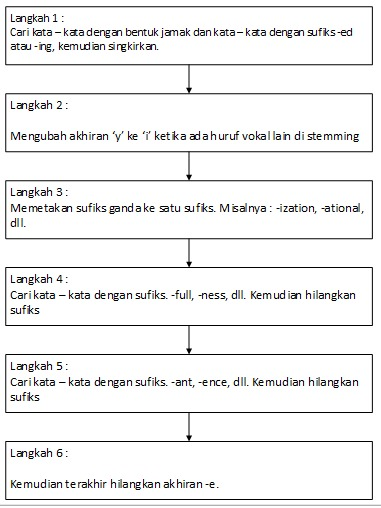
\includegraphics[width=6cm]{figures/porter_step.PNG}
        \caption{Non Linear
        \label{6step}}
        \end{figure} 
\begin{enumerate}
    \item Langkah 1 : hilangkan sufiks –ed dan –ing.
\begin{table}[!ht]
\centering
\begin{tabular}{|l|l|l|}
\hline
Kata-kata & Peraturan  & Hasil \\ \hline
\begin{tabular}[c]{@{}l@{}}amaze, amazed,\\ amazedly, amazedness\end{tabular} & \begin{tabular}[c]{@{}l@{}}-ly dan -ed\\ -ss dan -ed\end{tabular}   & amaz, amaz, amaz, amaz \\ \hline
\begin{tabular}[c]{@{}l@{}}amazing, amazingly, \\ amazingness\end{tabular}    & \begin{tabular}[c]{@{}l@{}}-ly dan -ing\\ -ss dan -ing\end{tabular} & amaz, amaz, amaz       \\ \hline
\end{tabular}
\end{table}
\vspace{3cm}

    \item Langkah 2 : mengubah sufiks `y` ke `i`.
\begin{table}[!ht]
\centering
\begin{tabular}{|l|l|l|}
\hline
Kata-kata & Peraturan & Hasil \\ \hline
cry       & -y ke -i  & cri   \\ \hline
dry       & -y ke -i  & dri   \\ \hline
\end{tabular}
\end{table}

    \item Langkah 3 : Memetakan sufiks ganda ke sufiks \textit{single}.
\begin{table}[!ht]
\centering
\begin{tabular}{|l|l|l|}
\hline
Kata-kata & Peraturan          & Hasil  \\ \hline
national  & -ational ke -ation & nation \\ \hline
\end{tabular}
\end{table}

    \item Langkah 4 : hilangkan sufiks -ness dan -full.
\begin{table}[!ht]
\centering
\begin{tabular}{|l|l|l|}
\hline
Kata-kata & Peraturan          & Hasil  \\ \hline
kindess  & -ness - & kind \\ \hline
\end{tabular}
\end{table}

    \item Langkah 5 : hilangkan sufiks -ant, -ance dan -ence.
\begin{table}[!ht]
\centering
\begin{tabular}{|l|l|l|}
\hline
Kata-kata & Peraturan          & Hasil  \\ \hline
compliance  & -ance - & compli \\ \hline
\end{tabular}
\end{table}

    \item Langkah 6 : hilangkan sufiks -e.
\begin{table}[!ht]
\centering
\begin{tabular}{|l|l|l|}
\hline
Kata-kata & Peraturan          & Hasil  \\ \hline
engine  & -e - & engin \\ \hline
\end{tabular}
\end{table}

\end{enumerate}


\section{Metode \textit{Naïve Bayes Classifier}}
\textit{Naïve Bayes Classifier} merupakan sebuah metoda klasifikasi yang berakar pada teorema Bayes. Metode pengklasifikasian dengan menggunakan metode probabilitas dan statistik yang dikemukakan oleh ilmuwan Inggris Thomas Bayes, yaitu memprediksi peluang di masa depan berdasarkan pengalaman di masa sebelumnya sehingga dikenal sebagai Teorema Bayes. Ciri utama dari \textit{Naïve Bayes Classifier} ini adalah asumsi yang sangat kuat akan independens dari masing-masing kondisi atau kejadian.
\par Menurut Olson dan Delen menjelaskan \textit{Naïve Bayes} untuk setiap kelas keputusan, menghitung probabilitas dengan syarat bahwa kelas keputusan adalah benar, mengingat vektor informasi obyek. Algoritma ini mengasumsikan bahwa atribut obyek adalah independen. Probabilitas yang terlibat dalam memproduksi perkiraan akhir dihitung sebagai jumlah frekuensi dari "\textit{master}" tabel keputusan.
\par Keuntungan penggunan adalah bahwa metoda ini hanya membutuhkan jumlah data pelatihan (\textit{training data}) yang kecil untuk menentukan estimasi parameter yang diperlukan dalam proses pengklasifikasian. Karena yang diasumsikan sebagai variable \textit{independent}, maka hanya varians dari suatu variable dalam sebuah kelas yang dibutuhkan untuk menentukan klasifikasi, bukan keseluruhan dari matriks kovarians.


\par \textbf{Kekurangan Metode \textit{Naïve Bayes Classifier}:}
\begin{enumerate}
    \item 	Tidak berlaku jika probabilitas kondisionalnya adalah nol, apabila nol maka probabilitas prediksi akan bernilai nol juga.
	\item Mengasumsikan variabel bebas.
\end{enumerate}

\par \textbf{Kelebihan Metode \textit{Naïve Bayes Classifier}:}
\begin{enumerate}
    \item Menangani kuantitatif dan data diskrit
    \item Kokoh untuk titik noise yang diisolasi, misalkan titik yang dirata – ratakan ketika mengestimasi peluang bersyarat data.
    \item Hanya memerlukan sejumlah kecil data pelatihan untuk mengestimasi parameter (rata-rata dan variansi dari variabel) yang dibutuhkan untuk klasifikasi.
    \item Menangani nilai yang hilang dengan mengabaikan instansi selama perhitungan estimasi peluang.
    \item Cepat dan efisiensi ruang.
	\item Kokoh terhadap atribut yang tidak relevan.
\end{enumerate}

\par \textbf{Naive Bayes} merupakan sebuah pengklasifikasian probabilistik sederhana yang menghitung sekumpulan probabilitas dengan menjumlahkan frekuensi dan kombinasi nilai dari dataset yang diberikan. Suatu metode yang dapat memprediksi probabilitas keanggotaan kelas suatu data yang akan masuk ke dalam kelas atau kategori tertentu, sesuai dengan perhitungan probabilitas.
\par \textbf{Naïve bayes} dapat digunakan untuk berbagai macam keperluan antara lain untuk klasifikasi dokumen, deteksi spam atau filtering spam, dan masalah klasifikasi lainnya. Pada penelitian ini terdapat Data Latih atau \textbf{Training} dan Data Uji atau \textbf{Testing}.\textbf{ Data Training} menggunakan data yang sebelumnya sudah diinputkan ke dalam aplikasi CMS, kemudian dicari seberapa sering sebuah kata masuk kedalam suatu kategori. Data Uji atau \textbf{Data Testing} adalah data yang akan diuji dan menggunakan perhitungan, kemudian dicari nilai probabilitasnya menggunakan teorema bayes. Teorema bayes merupakan dasar aturan dari \textbf{naive bayes classifier} berikut teorema bayes akan disajikan rumus berikut \ref{nbr}:
\begin{equation}
\label{nbr}
    P(W\_n|V\_n) = \frac{(n\_k + 1)}{(jumlah frekuensi + jumlah kata)} 
\end{equation} 
\par Keterangan \ref{nbr}:
\par P(W\_k|V\_j) adalah Probabilitas bobot setiap kategori
\par n\_k adalah Nilai kemunculan frekuensi kata
\par jumlah frekuensi adalah Jumlah Kemunculan kata pada setiap kategori
\par jumlah kata adalah Jumlah keseluruhan kata pada 

\par Berdasarkan rumus \ref{nbr} akan didapatkan probabilitas setiap kategori yang kemudian akan hitung probabilitas kategori dengan menggunakan rumus sebagai berikut pada \ref{nbb}

\begin{equation}
\label{nbb}
    P(V_j) = \frac{a}{b} 
\end{equation} 

\par Keterangan \ref{nbb}:
\par P(V\_j) adalah Probabilitas Kata
\par a adalah Jumlah dokumen pada setiap kategori
\par b adalah Jumlah total keseluruhan dokumen pada data training

\par Setelah itu, setiap kata pada judul dokumen akan dihitung dan dijumlahkan kemudian dihitung probabilitasnya. Kemudian dicari probabilitas mana yang paling besar, maka judul tersebut akan otomatis ke kategori yang memiliki nilai probabilitas tertinggi

\subsection{Contoh Kasus}
Perhitungan dengan menggunakan metode Naïve Bayes Classifier ada proses perhitungan mencari nilai probabilitas yang paling tinggi. Proses ini adalah menghitung setiap kata berdasarkan jumlah kata yang sering muncul pada sebuah kategori. Semakin sering sebuah kata di dalam judul maka nilai probabilitas terhadap kategori tersebut akan semakin tinggi. Penelitian ini menggunakan sebanyak 183 judul dokumen dibagi menjadi 9 kategori. Judul–judul dokumen tersebut didapatkan dari aplikasi CMS sebelumnya dan dijadikan sebagai data training untuk penelitian ini. Berikut 9 kategori judul dokumen:
    \begin{enumerate}
        \item 	Certification Management: Mengolah dokumen tentang sertifikasi dan izin terbang
    	\item Flight Test : Mengolah dokumen hasil tes terbang suatu pesawat.
	    \item Performance \& Stability : Mengolah dokumen performa stabilnya mesin pesawat.
	    \item Structure : Mengolah dokumen struktur mesin, cara kerja bagian sebuah pesawat.
        \item Mechanical \& Hydrouling : mengolah dokumen hydraulic.
    	\item Electrical System : Mengolah dokumen tentang elektrik dan kelistrikan pesawat.
	    \item Avionic System : Mengolah dokumen test fungsi bagian pesawat.
	    \item Propulsion \& Fuel System : Mengolah dokumen bahan bakar.
	    \item Interior and Cabin Safety : Mengolah dokumen design interior cabin suatu pesawat
    \end{enumerate}
    Berikut pada tabel \ref{tab:a} adalah kata kunci dari setiap kategori yang melewati tahap data training:
    \begin{table}[!ht]
    \caption{Tabel Kategori Kata Kunci}
    \label{tab:a}
    \centering
\begin{tabular}{|l|l|}
\hline
Kategori                  & Kata Kunci                                                                                                  \\ \hline
Certification Management  & \begin{tabular}[c]{@{}l@{}}Plan,  Certification, Modification, List, Configuration\end{tabular}          \\ \hline
Flight Test               & \begin{tabular}[c]{@{}l@{}}Flight,  Test, Certification, Result\end{tabular}                             \\ \hline
Performance \& Stability  & \begin{tabular}[c]{@{}l@{}}Engineering,  Justification, Performance, Qualities\end{tabular}              \\ \hline
Structure                 & \begin{tabular}[c]{@{}l@{}}Analysis,   Stress, Strenght, Load\end{tabular}                                \\ \hline
Mechanical \& Hydrouling  & \begin{tabular}[c]{@{}l@{}}Hydraulic,  Power, Technical\end{tabular}                                     \\ \hline
Electrical System         & \begin{tabular}[c]{@{}l@{}}Electrical,   Lighting, Subsystem\end{tabular}                                 \\ \hline
Avionic System            & \begin{tabular}[c]{@{}l@{}}Test,   Ground, Result, Procedure, Communication, \\Record, Require\end{tabular} \\ \hline
Propulsion \& Fuel System & \begin{tabular}[c]{@{}l@{}}Fuel,   Hazard, Functional\end{tabular}                                        \\ \hline
Interior and Cabin Safety & \begin{tabular}[c]{@{}l@{}}Interior,   Design, Cooling, Cabin, Air Conditioner\end{tabular}               \\ \hline
\end{tabular}
\end{table}

\par Kemudian setelah data training di dapatkan, maka selanjutnya adalah langkah pengujian. Dalam langkah pengujian ini maka akan dijumlahkan nilai probabilitas setiap kata pada setiap kategori kemudian dikalikan dengan probabilitas dokumen yang sudah dihitung. Untuk pengujian, akan dihitung dengan judul dokumen baru yang belum diketahui kategorinya. Judul dokumennya adalah : CN235-220M NAU5 List Of Procedure Certification Plan. Maka langkah pertama adalah melalui proses text mining yaitu preprocessing, kata kata yang di dapat adalah sebagai berikut.
\begin{table}[!ht]
\centering
\caption{Tabel Frekuensi Kemunculan Kata}
\begin{tabular}{|l|l|}
\hline
Kata     & Frekuensi \\ \hline
List     & 1         \\ \hline
Proced   & 1         \\ \hline
Certific & 1         \\ \hline
Plan     & 1         \\ \hline
\end{tabular}
\end{table}

\par Pada tabel 1 di dapat banyak frekuensi kemunculan kata pada judul dokumen baru atau data uji, kemudian akan dihitung nilai probabilitasnya pada setiap kategorinya. 
\begin{enumerate}
    \item Kategori 1 – Management
    \begin{table}[!ht]
\begin{tabular}{llll}
\multicolumn{2}{l}{\begin{tabular}[c]{@{}l@{}}P(list |\\ Management)\end{tabular}}     & \multicolumn{2}{l}{= (0+1) : (71) = 0.0141}                                                                         \\
\multicolumn{2}{l}{P(proced | Management)}                                             & \multicolumn{2}{l}{= (0+1) : (71) = 0.0141}                                                                         \\
\multicolumn{2}{l}{\begin{tabular}[c]{@{}l@{}}P(certific |\\ Management)\end{tabular}} & \multicolumn{2}{l}{= (2+1) : (71) = 0.0422}                                                                         \\
\multicolumn{2}{l}{\begin{tabular}[c]{@{}l@{}}P(plan |\\ Management)\end{tabular}}     & \multicolumn{2}{l}{= (2+1) : (71) = 0.0422}                                                                         \\
                                 & Jadi P(|Management)                                 & \multicolumn{2}{l}{0.0141 x 0.141 x 0.0422 x 0.0422}                                                                \\
                                 &                                                     & \multicolumn{2}{l}{= 0.000003540488004}                                                                             \\
                                 & Probabilitas                                        & \multicolumn{2}{l}{\begin{tabular}[c]{@{}l@{}}= P(Management)\\ x P(|Management)\end{tabular}}                      \\
                                 &                                                     & \multicolumn{2}{l}{= 0.11 x 0.000003540488004}                                                                      \\
                                 &                                                     & \multicolumn{2}{l}{\begin{tabular}[c]{@{}l@{}}0.00000038945368044 = \\ 3.8945 x 10$^-7$
                                 \end{tabular}}
\end{tabular}
\end{table}

\item 	Kategori 2 – Flight Test
\begin{table}[!ht]
\begin{tabular}{llll}
\multicolumn{2}{l}{\begin{tabular}[c]{@{}l@{}}P(list |\\ Flight)\end{tabular}}     & \multicolumn{2}{l}{= (0+1) : (76) = 0.0132}                                          \\
\multicolumn{2}{l}{P(proced | Flight)}                                             & \multicolumn{2}{l}{= (0+1) : (76) = 0.0132}                                          \\
\multicolumn{2}{l}{\begin{tabular}[c]{@{}l@{}}P(certific |\\ Flight)\end{tabular}} & \multicolumn{2}{l}{= (0+1) : (76) = 0.0132}                                          \\
\multicolumn{2}{l}{\begin{tabular}[c]{@{}l@{}}P(plan |\\ Flight)\end{tabular}}     & \multicolumn{2}{l}{= (0+1) : (76) = 0.0132}                                          \\
                                 & Jadi P(|Flight)                                 & \multicolumn{2}{l}{= 0.0132 x 0.0132 x 0.0132 x 0.0132}                              \\
                                 &                                                 & \multicolumn{2}{l}{= 0.0000000303595776}                                             \\
                                 & Probabilitas                                    & \multicolumn{2}{l}{\begin{tabular}[c]{@{}l@{}}P(Flight)\\ x P(|Flight)\end{tabular}} \\
                                 &                                                 & \multicolumn{2}{l}{0.11 x 0.0000000303595776}                                        \\
                                 &                                                 & \multicolumn{2}{l}{= 0.000000003339553536 = 3.33955 x 10\textasciicircum{}-9}       
\end{tabular}
\end{table}

\item 	Kategori 3 – Performance 
\begin{table}[!ht]
\begin{tabular}{llll}
\multicolumn{2}{l}{\begin{tabular}[c]{@{}l@{}}P(list |\\ Performance)\end{tabular}}    & \multicolumn{2}{l}{= (0+1) : (76) = 0.0132}                                                    \\
\multicolumn{2}{l}{P(proced | Performance)}                                            & \multicolumn{2}{l}{= (0+1) : (76) = 0.0132}                                                    \\
\multicolumn{2}{l}{\begin{tabular}[c]{@{}l@{}}P(certific |\\ Performance\end{tabular}} & \multicolumn{2}{l}{= (0+1) : (76) = 0.0132}                                                    \\
\multicolumn{2}{l}{\begin{tabular}[c]{@{}l@{}}P(plan |\\ Performance)\end{tabular}}    & \multicolumn{2}{l}{= (0+1) : (76) = 0.0132}                                                    \\
                                 & Jadi P(|Performance)                                & \multicolumn{2}{l}{= 0.0132 x 0.0132 x 0.0132 x 0.0132}                                        \\
                                 &                                                     & \multicolumn{2}{l}{= 0.0000000303595776}                                                       \\
                                 & Probabilitas                                        & \multicolumn{2}{l}{\begin{tabular}[c]{@{}l@{}}P(Performance)\\ x P(|Performance)\end{tabular}} \\
                                 &                                                     & \multicolumn{2}{l}{0.11 x 0.0000000303595776}                                                  \\
                                 &                                                     & \multicolumn{2}{l}{= 0.000000003339553536 = 3.33955 x 10\textasciicircum{}-9}                 
\end{tabular}
\end{table}

\end{enumerate}

\par Dari perhitungan diatas, didapatkan hasil probabilitas dari setiap kategori, berikut adalah hasil probabilitas dari setiap kategori.

\begin{table}[]
\centering
\begin{tabular}{|l|l|}
\hline
Kategori                                                          & Hasil                            \\ \hline
1 – Management                                                    & 3.8945 x 10\textasciicircum{}-7  \\ \hline
\begin{tabular}[c]{@{}l@{}}2 – Flight\\   Test\end{tabular}       & 3.8955 x 10\textasciicircum{}-9  \\ \hline
\begin{tabular}[c]{@{}l@{}}3 –\\   Performance\end{tabular}       & 3.8955 x 10\textasciicircum{}-9  \\ \hline
4 -  Structure                                                    & 3.8703 x 10\textasciicircum{}-9  \\ \hline
\begin{tabular}[c]{@{}l@{}}5 - Mechanical\\   System\end{tabular} & 7.75006 x 10\textasciicircum{}-9 \\ \hline
6 – Electrical                                                    & 4.1063 x 10\textasciicircum{}-9  \\ \hline
7 – Avionic                                                       & 3.87503 x 10\textasciicircum{}-9 \\ \hline
8 – Propulsion                                                    & 3.65366 x 10\textasciicircum{}-9 \\ \hline
\begin{tabular}[c]{@{}l@{}}9 – Cabin\\   Safety\end{tabular}      & 4.1063 x 10\textasciicircum{}-9  \\ \hline
\end{tabular}
\end{table}

\par Jadi dapat dilihat bahwa dokumen dengan judul “CN235-220M NAU5 List Of Procedure Certification Plan” setelah melalui peroses text preprocessing dengan Algoritma Porter dan Metode NBC termasuk ke kategori Management karena memiliki probabilitas paling tinggi yaitu 3.8945 x 10-7.

% =============================Boby J,H====================================

\section{Metode TF-IDF}
\subsection{Pengertian Metode TF-IDF}
TF-IDF adalah metode pembobotan yang
paling umum digunakan untuk menggambarkan
dokumen dalam vector space model. Dalam
klasifikasi teks, fungsi pembobotan ini terkait
dengan dua metode pembelajaran yang penting
yaitu k-NN dan SVM. TF-IDF umumnya
digunakan untuk membandingkan vektor query
dengan vektor dokumen menggunakan
kesamaan (similarity).
Term Frequency (TF) adalah faktor yang
menentukan bobot term pada suatu dokumen
berdasarkan jumlah kemunculannya dalam
dokumen tersebut. Nilai kumlah kemunculan
suatu kata (term frequency) diperhitungkan
dalam pemberian bobot terhadap suatu kata
(term frequency) diperhitungkan dalam
pemberian bobot terhadap suatu kata. Semakin
besar jumlah kemunculan suatu term dalam
dokumen, semakin besar pula bobotnya dalam
dokumen atau akan memberikan nilai
kesesuaian yang semakin besar.
Inverse Document Frequency (IDF) adalah
pengurangan dominasi term yang sering muncul
di berbagai dokumen. Hal ini diperlukan karena
term yang banyak muncul di berbagai
dokumen, dapat dianggap sebagai term umum
(common term) sehingga tidak penting nilainya.
Sebaliknya faktor kejarangmunculan kata (term
scarcity) dalam koleksi dokumen harus
diperhatikan dalam pemberian bobot. Kata yang
muncul pada sedikit dokumen harus dipandang
sebagai kata yang lebih penting (uncommon
term) daripada kata yang muncul pada banyak
dokumen. Pembobotan akan memperhitungkan
faktor kebalikan frekuensi dokumen yang
mengandung suatu kata (inverse document
frequency). Hal ini merupakan usulan dari
George Zipf. Zipf mengamati bahwa frekuensi
dari sesuatu cenderung kebalikan secara
proposional dengan urutannya.

\subsection{Kelebihan Metode TF-IDF}
Metode TF/IDF dikenal sebagai algorithma yang sederhana namun relevan dalam melakukan pencocokan kata pada sebuah dokumen.
\subsection{Kekurangan Metode TF-IDF}
penggunaan fitur urutan kata dalam pembobotan masih memiliki kekurangan.
Hal tersebut dikarenakan contohnya terdapat beberapa dokumen yang sangat panjang namun tidak relevan. Dokumendokumen ini biasanya melakukan banyak perulangan kata-kata. Sebaliknya, terdapat dokumen yang pendek namun di dalamnya memuat informasi yang penting sehingga urutan kata query yang ada dalam dokumen tersebut lebih sedikit. Oleh karena itu, diperlukan proses penyesuaian terhadap fitur urutan kata tersebut dengan melibatkan fitur panjang dokumen sehingga dokumen yang diha
\subsection{Penjelasan Metode TF-IDF}
Formula yang digunakan untuk menghitung bobot (w) masing-masing dokumen terhadap kata kunci adalah 
\begin{equation}
    Wdt = tfdt *Idft
\end{equation}
Dimana :
\begin{itemize}
    \item Wdt= bobot dokumen ke­d terhadap kata ke­t  
    \item tfdt = banyaknya kata yang dicari pada sebuah 
dokumen  
    \item Idft = Inversed Document Frequency (log 
(N/df) )
    \item N = total dokumen  
    \item df = banyak dokumen yang mengandung kata 
yang dicari.
\end{itemize}

Setelah bobot (w) masing-masing dokumen diketahui, maka dilakukan proses \textit{sorting}/pengurutan dimana semakin besar nilai w, semakin besar tingkat similaritas dokumen tersebut kata yang dicari, demikian sebaliknya.

\subsection{Penerapan Metode TF-IDF}
Berikut dibawah ini diberikan contoh kasus perhitungan bobot dokumen terhadap query, dengan menggunakan metTF-IDF.
\subsubsection{Contoh Soal 1}
\par Contoh query: gold silver truck. Sehingga didapatkan query terms (Q):
\begin{itemize}
    \item gold
    \item silver
    \item truck
\end{itemize}

Untuk koleksi dokumen nya terdapat:
\begin{itemize}
    \item dokumen 1 \textbf{(d1)} = Shipment of gold damaged in a fire
    \item dokumen 2 \textbf{(d2)} = Delivery of silver arrived in a silver truck
    \item dokumen 3 \textbf{(d3)} = Shipment of gold arrived in a truck
\end{itemize}

\par Jadi total jumlah dokumen dalah koleksi dokumen \textbf{(D) = 3}\\

\par Untuk setiap query dan dokumen dalam koleksi, dilakukan pemotongan string berdasarkan tiap kata yang menyusunnya, menghilangkan tanda baca, angka dan stopword.

\par Setelah melalui proses ini, maka kata \textbf{“of”}, \textbf{“in”}, dan \textbf{“a”} pada ketiga dokumen dihapus lalu di-stemming sehingga didapatkan term-term (documents terms) sebagai berikut:\\

\textbf{– ship – gold – damage – fire – deliver – silver – arrive – truck} \\

Tahapan proses keseluruhan diatas dinamakan preprocessing text.
\par Pada tahap selanjutnya tiap dokumen diwujudkan sebagai sebuah vektor dengan elemen sebanyak term query yang terdapat dalam tiap dokumen yang berhasil dikenali dari tahap ekstraksi dokumen sebelumnya. Vektor tersebut beranggotakan bobot dari setiap term query yang dihitung berdasarkan metode TF-IDF.

\begin{figure}[!htbp]
\centering
\includegraphics[scale=0.6]{chapters/figures/diagram1.JPG}
    \label{Figure4}
    \caption{Daigram Representasi Term Query Pada Ruang Vektor}
\end{figure}

\par Fungsi metode ini adalah untuk mencari representasi nilai dari tiap dokumen dalam koleksi. Dari sini akan dibentuk suatu vektor antara dokumen dan query yang ditentukan oleh nilai bobot term query dalam dokumen.

\par Semakin besar nilai perhitungan bobot yang diperoleh maka semakin tinggi tingkat similaritas dokumen terhadap query. Contohnya untuk perhitungan bobot \textbf{(w)} term query silver dalam dokumen 2 \textbf{(d2)} = Delivery of silver arrived in a silver truck, yaitu: jumlah kemunculan term silver dalam dokumen 2 \textbf{(d2)} adalah sebanyak dua kali \textbf{(tf = 2)}, total dokumen yang ada di koleksi sebanyak tiga dokumen \textbf{(D)=3}, dari ketiga dokumen dalam koleksi, term silver muncul pada dokumen 2 \textbf{(d2)} saja, sehingga total dokumen yang mengandung term silver adalah satu dokumen \textbf{(df)=1}, sehingga dapat diperoleh nilai bobot term silver pada dokumen 2 \textbf{(d2)}
\begin{equation}
    W ij = tfij xlog(D/dfi) + 1
\end{equation}
\begin{equation}
    W ij = 2 x (log(3/1) + 1
\end{equation}
\begin{equation}
    W ij = 2 x (0.477 + 1)
\end{equation}

\par Dengan demikian dapat diperoleh nilai bobot (w) untuk setiap term pada query dalam masing-masing dokumen: 

\begin{table}[]
\centering
\caption{Data Jarak Dari Titik Awal}
\begin{tabular}{|l|l|l|l|l|l|l|l|l|l|}
\hline
Q      & d1 & d2 & d3 & df & IDF   & IDF+1 & D1    & D2    & D3    \\ \hline
GOLD   & 1  & 0  & 1  & 2  & 0.176 & 0.176 & 1.176 & 0     & 1.176 \\ \hline
SILVER & 0  & 2  & 0  & 1  & 0.477 & 1.477 & 0     & 2.954 & 0     \\ \hline
TRUCK  & 1  & 1  & 1  & 2  & 0.176 & 1.176 & 0     & 1.176 & 1.176 \\ \hline
       &    &    &    &    &       &       & 1.176 & 4.130 & 2.352 \\ \hline
\end{tabular}
\end{table}

\section{K-Nearest Neighbor (KNN)}
\par K-Nearest Neighbor (KNN) adalah metode melakukan klasifikasi terhadap objek
berdasarkan data pembelajaran yang jaraknya paling dekat dengan objek tersebut. Metode ini bertujuan untuk mengklasifikasikan objek baru berdasarkan atribut dan training sample.
Diberikan suatu titik query, selanjutnya akan ditemukan sejumlah K objek atau titik training yang paling dekat dengan titik query. Nilai prediksi dari query akan ditentukan berdasarkan klasifikasi tetanggaan. \par 
Algoritma K-Nearest Neighbor (KNN) adalah sebuah metode untuk melakukan klasifikasi terhadap objek berdasarkan data pembelajaran yang jaraknya paling dekat dengan objek tersebut. 
Teknik ini sangat sederhana dan mudah diimplementasikan. Tahapannya sebegai berikut :
\newpage
\begin{figure}
    \centering
    \centerline{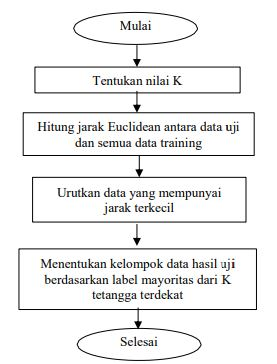
\includegraphics[width=0.60\textwidth]{chapters/figures/metodeknn.JPG}}
    \caption{Proes Metode K Nearest Neighbor}
    \label{fig:my_label}
\end{figure}

Mirip dengan teknik clustering, yaitu mengelompokkan suatu data baru berdasarkan jarak data baru itu ke beberapa data/tetangga terdekat. Pertama sebelum mencari jarak data ke tetangga adalah menentukan nilai K tetangga (neighbor). Lalu, untuk mendefinisikan jarak antara dua titik yaitu titik pada data training dan titik pada data testing, maka digunakan rumus Euclidean dengan persamaan \ref{knn1}, sebagai berikut:
\\
\begin{equation}
\label{knn1}
    d(a, b) =\sum^n _i=0 (Xi-Yi)^2
\end{equation}
\par Keterangan:
\begin{itemize}
    \item d (a,b) : jarak Euclidian
    \item x : data 1
    \item y : data 2
    \item i : fitur ke -
    \item n : jumlah fitur
\end{itemize}

\subsection{Tahapan Langkah Algoritma K-NN}
\begin{enumerate}
    \item Menentukan parameter k (jumlah tetangga paling dekat).
    \item Menghitung kuadrat jarak eucliden objek terhadap data training yang diberikan.
    \item Mengurutkan hasil no 2 secara ascending (berurutan dari nilai tinggi ke rendah)
    \item Mengumpulkan kategori Y (Klasifikasi nearest neighbor berdasarkan nilai k)
    \item Dengan menggunakan kategori nearest neighbor yang paling mayoritas maka dapat dipredisikan kategori objek.
\end{enumerate}
\subsection{Kelebihan K-Nearest Neighbor (KNN)}
KNN memiliki beberapa kelebihan yaitu :
\begin{enumerate}
    \item Sangat nonlinear
    \item Mudah dipahami dan diimplementasikan
    \item tangguh terhadap training data yang noisy dan efektif apabila data latih nya besar.
\end{enumerate}

\subsection{Kekurangan K-Nearest Neighbor (KNN)}
KNN memiliki beberapa kekurangan yaitu :
\begin{enumerate}
    \item Tidak menangani nilai hilang (missing value) secara implisit
    \item Sensitif terhadap data pencilan (outlier)
    \item Perlu menentukan nilai dari parameter K (jumlah dari tetangga terdekat)
    \item Rentan terhadap variabel yang non-informatif
    \item Rentan terhadap dimensionalitas yang tinggi
    \item Rentan terhadap perbedaan rentang variabel
    \item Nilai komputasi yang tinggi
    \item Pembelajaran berdasarkan jarak tidak jelas
\end{enumerate}

\subsection{Penerapan K-Nearest Neighbor (KNN)}
\par Terdapat beberapa data yang berasal dari survey questioner tentang klasifikasi kualitas kertas tissue apakah baik atau jelek, dengan objek training dibawah ini menggunakan dua attribute yaitu daya tahan terhadap asam dan kekuatan.
\newpage
\begin{table}[]
\centering
\caption{Contoh perhitungan k-nn}
\begin{tabular}{|l|l|l|}
\hline
\begin{tabular}[c]{@{}l@{}}X1 = Daya \\ tahan asam \\ (Detik\end{tabular} & \begin{tabular}[c]{@{}l@{}}X2 = \\ Kekuatan\\ (kg/m2)\end{tabular} & \begin{tabular}[c]{@{}l@{}}Y = \\ Klasifikasi\end{tabular} \\ \hline
8                                                                         & 4                                                                  & Baik                                                       \\ \hline
4                                                                         & 5                                                                  & Jelek                                                      \\ \hline
4                                                                         & 6                                                                  & Jelek                                                      \\ \hline
7                                                                         & 7                                                                  & Baik                                                       \\ \hline
5                                                                         & 6                                                                  & Jelek                                                      \\ \hline
6                                                                         & 5                                                                  & Baik                                                       \\ \hline
\end{tabular}
\end{table}

\par Akan diproduksi kembali kertas tissue dengan attribute \textbf{X1=7} dan \textbf{X2=4}, tanpa harus mengeluarkan biaya untuk melakukan survey, maka dapat diklasifikasikan kertas tissue tersebut termasuk yang baik atau jelek.
\newpage

\begin{table}[]
\centering
\caption{contoh perhitungan k-nn (2)}
\begin{tabular}{|l|l|l|}
\hline
X1 & X2 & \begin{tabular}[c]{@{}l@{}}Squere distance\\   to query distance \\ (7,4)\end{tabular} \\ \hline
8  & 4  & (8-7)\textasciicircum{}2+(4-4)\textasciicircum{}2=1                                    \\ \hline
4  & 5  & (4-7)\textasciicircum{}2+(5-4)\textasciicircum{}2=10                                   \\ \hline
4  & 6  & (4-7)\textasciicircum{}2+(6-4)\textasciicircum{}2=13                                   \\ \hline
7  & 7  & (7-7)\textasciicircum{}2+(7-4)\textasciicircum{}2=9                                    \\ \hline
5  & 6  & (5-7)\textasciicircum{}2+(6-4)\textasciicircum{}2=8                                    \\ \hline
6  & 5  & (6-7)\textasciicircum{}2+(5-4)\textasciicircum{}2=2                                    \\ \hline
\end{tabular}
\end{table}

\begin{table}[]
\centering
\caption{contoh perhitungan k-nn (3)}
\begin{tabular}{|l|l|l|l|l|}
\hline
X1 & X2 & Jarak Terkecil & K     & Y     \\ \hline
8  & 4  & 1              & Ya    & Baik  \\ \hline
4  & 5  & 5              & Tidak & -     \\ \hline
4  & 6  & 6              & Tidak & -     \\ \hline
7  & 7  & 4              & Ya    & Baik  \\ \hline
5  & 6  & 3              & Ya    & Jelek \\ \hline
6  & 5  & 2              & Ya    & Baik  \\ \hline
\end{tabular}
\end{table}

\par Dengan mengurutkan jarak terkecil, semisal diambil K=3, maka perbandingan nya adalah 2 (Baik) >1 (Jelek). Maka dapat disimpulkan kertas tissue dengan attribute \textbf{X1=7} dan \textbf{X2=4} masuk ke kelas \textbf{Baik}.
